%%%%%%%%%%%%%%%%%%%%%%%%%%%%%%%%%%%%%%%%%%%%%%%%%%%
%% Rapport — Chapitre 6 : Algorithmes Quantiques
%% Stage LIA / CERI — Université d'Avignon
%% Stagiaire : Patrice SEBASTIANO
%% Encadrant : Serigne GUEYE
%%%%%%%%%%%%%%%%%%%%%%%%%%%%%%%%%%%%%%%%%%%%%%%%%%%

\documentclass{ceri/sty/rapport}

%%%%%%%%%%%%%%%%%%%%%%%%%%%%%%%%%%%%%%%%%%%%%%%%%%%
%% Informations générales
%%%%%%%%%%%%%%%%%%%%%%%%%%%%%%%%%%%%%%%%%%%%%%%%%%%
\major{Master d'Informatique}
\specialization{Informatique Quantique}
\course{Stage de Recherche — LIA Avignon}

\title{Rapport — Chapitre 6}
\subtitle{Algorithmes Quantiques :\\Deutsch-Jozsa, Grover et Dürr-Høyer}
\author{Patrice SEBASTIANO}

\advisor[Encadrant]{Serigne GUEYE}

%%%%%%%%%%%%%%%%%%%%%%%%%%%%%%%%%%%%%%%%%%%%%%%%%%%
%% Packages supplémentaires
%%%%%%%%%%%%%%%%%%%%%%%%%%%%%%%%%%%%%%%%%%%%%%%%%%%
\usepackage{graphicx}
\usepackage{amsmath,amssymb}
\usepackage{mathtools}
\usepackage{braket}
\usepackage{quantikz}
\usepackage{tcolorbox}
\usepackage{listings}
\usepackage{booktabs}
\usepackage{xcolor}
\tcbuselibrary{breakable, skins}

\definecolor{codebg}{RGB}{245,245,245}
\definecolor{codeframe}{RGB}{180,180,180}

\lstset{
    language=Python,
    basicstyle=\ttfamily\small,
    keywordstyle=\bfseries\color{blue!70!black},
    commentstyle=\itshape\color{gray},
    stringstyle=\color{orange!80!black},
    backgroundcolor=\color{codebg},
    frame=single,
    rulecolor=\color{codeframe},
    breaklines=true,
    showstringspaces=false
}

%%%%%%%%%%%%%%%%%%%%%%%%%%%%%%%%%%%%%%%%%%%%%%%%%%%
%% Document
%%%%%%%%%%%%%%%%%%%%%%%%%%%%%%%%%%%%%%%%%%%%%%%%%%%
\renewcommand{\MyToc}{
    \tableofcontents
    \thispagestyle{fancy}
    \newpage
}
\makeatletter
\let\orig@maketitleZ\maketitleZ
\renewcommand{\maketitleZ}{
    \hypersetup{
        pdftitle={\MyTitle\ -- \MySubtitle},
        pdfauthor={\MyAuthor},
        pdfsubject={\MyCourse}
    }
    \setHeaders
    \begin{titlepage}
        \begin{tikzpicture}[remember picture,overlay]
            \node at (current page.south west)
            {   \begin{tikzpicture}[remember picture,overlay]
                    \newlength{\myYpos}
                    \useasboundingbox (0,0) rectangle(\the\paperwidth,\the\paperheight);
                    \node[anchor=north west, inner sep=-0.01cm] at (current page.north west){%
                        
\includegraphics{ceri/images/red_background.pdf}};
                    \pgftext[x=1cm, y=22.5cm, top, left]
                        {\parbox[t]{19cm}{\raggedright\fontsize{45}{45}{\textbbf{\textcolor{white}{\MyTitle}}}
                        \\[0.2cm] \fontsize{30}{30}{\textit{\textbbf{\textcolor{white}{\parbox[t]{19cm}{\raggedright\MySubtitle}}}}}}};
                    \setlength{\myYpos}{15.5cm}
                    \pgftext[x=1cm, y=\myYpos, top, left]
                        {\begin{minipage}{19cm}
                            \begin{doublespace}
                                \fontsize{20}{20}{\textbbf{\textcolor{white}{\MyAuthor}}}
                            \end{doublespace}
                        \end{minipage}};
                    \pgftext[x=20cm, y=\myYpos, top, right]
                        {\fontsize{20}{20}{\textbbf{\textcolor{white}{\mydate}}}};
                    \setlength{\myYpos}{8cm}
                    \pgftext[x=20cm, y=\myYpos, top, right]
                        {\begin{minipage}{19cm}
                            \raggedleft
                            \fontsize{16}{16}{\textbbf{\MyAdvisorTitle} \\ \textmd{\MyAdvisor \\}}
                        \end{minipage}};
                    \pgftext[x=1cm, y=\myYpos, top, left]
                        {\begin{minipage}{19cm}
                            \fontsize{16}{16}{
                            \raggedright
                            \textbbf{\MyMajor} \\
                            \textbbf{\MySpecialization} \\
                            \vspace{0.2cm}
                            \textbbf{UE}~\textmd{\MyCourse} \\
                            }\end{minipage}};
                \end{tikzpicture}
            };
        \end{tikzpicture}
    \end{titlepage}
    \setcounter{page}{2}
    \thispagestyle{fancy}
    \newpage
    \MyToc
}
\makeatother

\begin{document}

\maketitle
\sloppy

\setcounter{section}{5}
\section{Algorithmes Quantiques}
\label{sec:chap6}

Ce rapprot présente l'implémentation de deux algorithmes quantiques suivants : Deutsch-Jozsa et Grover, implémentés en Qiskit 2.x, accompagnée de leurs circuits dessinés en \LaTeX{} avec la bibliothèque \texttt{quantikz}.

%--------------------------------------------------
\subsection{Algorithme de Deutsch-Jozsa}
%--------------------------------------------------

\subsubsection{Problème}

Est donné une fonction booléenne $f : \{0,1\}^n \to \{0,1\}$, et les définitions suivantes :
\[
  f(x) = \begin{cases}
    c \in \{0,1\} & \forall\, x \in \{0,1\}^n
      \quad \textbf{(constante)} \\[6pt]
    0 \text{ ou } 1 \text{ avec }
      \bigl|\{x \mid f(x)=0\}\bigr| = \bigl|\{x \mid f(x)=1\}\bigr| = 2^{n-1}
      & \quad \textbf{(équilibrée)} \\[6pt]
    \text{ni constante ni équilibrée}
      & \quad \textbf{(autre)}
  \end{cases}
\]
Le but est de déterminer à quelle catégorie appartient $f$.

Un algorithme classique déterministe nécessite $2^{n-1}+1$ requêtes dans le pire
cas. L'algorithme de Deutsch-Jozsa répond en \textbf{une seule requête quantique}.

\subsubsection{Circuit}

\[
\begin{quantikz}
  \lstick{$\ket{0}^{\otimes n}$} & \gate{H^{\otimes n}} & \gate[wires=2]{O_f}
    & \gate{H^{\otimes n}} & \meter{} \\
  \lstick{$\ket{1}$} & \gate{H} & & \qw & \qw
\end{quantikz}
\]

Le registre ancilla est préparé dans $\ket{-}$ pour activer le \emph{phase
kickback}. Après l'oracle et la transformée de Hadamard inverse, la règle de
décision est :
\begin{gather*}
  \text{mesure} = \mathbf{0}^n \iff f \text{ est constante.} \\
  \text{mesure} \neq \mathbf{0}^n,\; \text{toutes mesures présentes} \iff f \text{ est équilibrée.} \\
  \text{sinon},\; f \text{ n'est ni constante ni équilibrée.}
\end{gather*}

\subsubsection{Implémentation}

L'implémentation teste toutes les fonctions binaires jusqu'à
$n = N_{\max} = 3$ bits. La valeur $N_{\max} = 4$ a été écartée car elle génère
$4^4 = 256$ oracles, ce qui demande un temps d'exécution trop long.

La partie critique est la génération procédurale des oracles.
\texttt{itertools.product([0,1], repeat=$2^n$)} énumère les $2^{2^n}$ tables de
vérité possibles. Pour chaque table, on construit le circuit correspondant.

La difficulté vient de la porte MCX : elle se déclenche uniquement quand
\emph{tous} ses qubits de contrôle valent $\ket{1}$. Or, $x$ est la représentation
binaire de l'indice de la ligne courante dans la table de vérité, et certains
de ses bits valent $0$. Pour chaque ligne où $f(x) = 1$, on applique une
porte $X$ sur chacun des qubits d'entrée dont le bit correspondant dans $x$
vaut $0$ (ce qui les amène à $\ket{1}$, permettant le déclenchement de la MCX),
puis on remet ces mêmes qubits à $\ket{0}$ après la MCX pour ne pas corrompre
les autres termes de la superposition :

\begin{minipage}{\linewidth}
\begin{lstlisting}
def generate_oracles(n):
    for k, truth_table in enumerate(itertools.product([0,1], repeat=2**n)):
        qc = QuantumCircuit(n + 1, name=f"Oracle_f_{k}")
        target = n
        for x, fx in enumerate(truth_table):
            if fx == 1:
                bits = format(x, f'0{n}b')
                # flip qubits where bit=0 so MCX fires on this input
                for i, b in enumerate(reversed(bits)):
                    if b == '0':
                        qc.x(i)
                qc.mcx(list(range(n)), target)
                # uncompute
                for i, b in enumerate(reversed(bits)):
                    if b == '0':
                        qc.x(i)
\end{lstlisting}
\end{minipage}

\subsubsection{Résultats}

Le circuit a été exécuté sur les $2^{2^n}$ oracles pour $n \in \{1, 2, 3\}$.
Les résultats obtenus sont les suivants :

\begin{center}
\begin{tabular}{lrrr}
\toprule
 & $n=1$ & $n=2$ & $n=3$ \\
\midrule
Constantes  & 2  & 2  & 2   \\
Équilibrées & 2  & 6  & 70  \\
Autres      & 0  & 8  & 184 \\
\midrule
Total       & 4  & 16 & 256 \\
\bottomrule
\end{tabular}
\end{center}

Le nombre de fonctions constantes est toujours $2$ ($f \equiv 0$ et $f \equiv 1$),
quel que soit $n$. Le nombre de fonctions équilibrées vaut $\binom{2^n}{2^{n-1}}$
(choisir quelles $2^{n-1}$ entrées reçoivent la valeur $1$), ce qui donne bien
$2$, $6$ et $70$ pour $n = 1, 2, 3$. Toutes les autres fonctions sont classifiées
dans la catégorie \textit{autre} — elles ne sont ni constantes ni équilibrées,
et l'algorithme de Deutsch-Jozsa les détecte correctement comme telles.

\newpage
%--------------------------------------------------
\subsection{Algorithme de Grover}
%--------------------------------------------------

\subsubsection{Problème}

On dispose d'une liste non ordonnée de $N = 2^n$ entiers stockés dans un
DataFrame Pandas. On cherche l'indice $i^*$ d'une valeur cible $v^*$.
L'algorithme de Grover résout ce problème en $O(\sqrt{N})$ requêtes, alors qu'en informatique classique, il faut $O(N)$ dans le pire des cas.

\subsubsection{Structure des registres}

Le circuit utilise quatre registres :

\begin{center}
\begin{tabular}{llp{7cm}}
\toprule
Registre & Taille & Rôle \\
\midrule
\texttt{idx} & $n$ qubits & Superposition des indices — mesuré en sortie \\
\texttt{val} & $n_{\mathrm{val}}$ qubits & Représentation binaire de $v_i$ — intriqué avec \texttt{idx} lors du chargement \\
\texttt{anc} & $n_{\mathrm{val}}$ qubits & Ancilla pour la comparaison bit à bit \\
\texttt{tgt\_phase} & 1 qubit & Préparé dans $\ket{-}$ pour le phase kickback \\
\bottomrule
\end{tabular}
\end{center}

\subsubsection{Vue d'ensemble du circuit}

\[
\begin{quantikz}
  \lstick{$idx$}  & \gate{H} & \qw
    & \gategroup[4,steps=5,style={dashed,rounded corners}]
        {R\'ep\'eter \ensuremath{\approx\!\sqrt{N}} fois}
      \qw
    & \gate[wires=2]{\shortstack{Load\\Data}}
    & \qw
    & \gate[wires=2]{\shortstack{Unload\\Data}}
    & \gate{\shortstack{Grover\\Diff.}}
    & \meter{} \\
  \lstick{$val$}  & \qw & \qw & \qw
    &
    & \gate[wires=3]{\shortstack{NOT-XOR\\Oracle}}
    &
    & \qw & \qw \\
  \lstick{$anc$}  & \qw & \qw & \qw & \qw
    &
    & \qw & \qw & \qw \\
  \lstick{$tgt$}  & \gate{X} & \gate{H} & \qw & \qw
    &
    & \qw & \qw & \qw
\end{quantikz}
\]

Le nombre d'itérations optimal est :
\[
  k = \left\lfloor \frac{\pi}{4} \sqrt{\frac{N}{k_{\mathrm{cibles}}}} \right\rfloor.
\]

\subsubsection{Encodage des données}

L'étape de chargement associe à chaque indice en superposition la valeur
correspondante dans la liste. Après cette étape, l'état du système est :
\[
  \frac{1}{\sqrt{N}} \sum_{i=0}^{N-1} \ket{i}\ket{v_i},
\]
ce qui constitue une \emph{représentation quantique du DataFrame} : chaque indice
$i$ est intriqué avec la valeur $v_i$ qui lui est associée.

\medskip
\textbf{Construction procédurale.}
Le circuit de chargement est généré dynamiquement à partir du DataFrame :
pour chaque ligne $i$, on applique une porte MCX par bit de $v_i$ égal à $1$,
contrôlée sur l'état $\ket{i}$ du registre \texttt{idx}.

Par exemple, pour la liste suivante (indice sur 2 bits, valeur sur 3 bits) :

\medskip
\noindent\makebox[\linewidth][c]{%
\begin{minipage}[c]{0.42\linewidth}
\centering
\begin{tabular}{cc@{\hspace{0.9em}}cc}
\toprule
\multicolumn{2}{c}{Indice} & \multicolumn{2}{c}{Valeur} \\
\cmidrule(r){1-2}\cmidrule(l){3-4}
déc & bin & déc & bin \\
\midrule
0 & 00 & 2 & 010 \\
1 & 01 & 5 & 101 \\
2 & 10 & 4 & 100 \\
3 & 11 & 7 & 111 \\
\bottomrule
\end{tabular}
\smallskip

{\small\textit{Données d'entrée}}
\end{minipage}%
\hspace{4em}%
\begin{minipage}[c]{0.42\linewidth}
\centering
\vspace{0.5em}
\[
  \frac{1}{2}\bigl(
    \ket{00}\ket{010} + \ket{01}\ket{101} +
    \ket{10}\ket{100} + \ket{11}\ket{111}
  \bigr)
\]
\vspace{-0.5em}
{\small\textit{État quantique après chargement}}
\end{minipage}%
}

\medskip\noindent
Les portes $X$ avant et après chaque MCX retournent temporairement les qubits de
contrôle à $\ket{1}$ pour les bits de l'indice qui valent $0$ :

\smallskip
\noindent\makebox[\linewidth][c]{%
\scalebox{0.82}{%
\begin{quantikz}[column sep=2pt]
  \lstick{$q_0$} & \gate{X} & \ctrl{3} & \gate{X} & \qw      & \ctrl{2} & \ctrl{4} & \qw      & \gate{X} & \ctrl{4} & \gate{X} & \ctrl{2} & \ctrl{3} & \ctrl{4} & \qw \\
  \lstick{$q_1$} & \gate{X} & \ctrl{2} & \gate{X} & \gate{X} & \ctrl{1} & \ctrl{3} & \gate{X} & \qw      & \ctrl{3} & \qw      & \ctrl{1} & \ctrl{2} & \ctrl{3} & \qw \\
  \lstick{$v_0$} & \qw      & \qw      & \qw      & \qw      & \targ{}  & \qw      & \qw      & \qw      & \qw      & \qw      & \targ{}  & \qw      & \qw      & \qw \\
  \lstick{$v_1$} & \qw      & \targ{}  & \qw      & \qw      & \qw      & \qw      & \qw      & \qw      & \qw      & \qw      & \qw      & \targ{}  & \qw      & \qw \\
  \lstick{$v_2$} & \qw      & \qw      & \qw      & \qw      & \qw      & \targ{}  & \qw      & \qw      & \targ{}  & \qw      & \qw      & \qw      & \targ{}  & \qw
\end{quantikz}
}%
}

\smallskip
\begin{center}
{\small\textit{Circuit de chargement des données pour les 4 indices}}
\end{center}

\smallskip
Chaque indice $\ket{i}$ est désormais intriqué avec la valeur $\ket{v_i}$
correspondante dans la liste.

\medskip
\textbf{Déchargement des données.}
Après l'oracle, le registre \texttt{val} doit être remis à $\ket{0}$, faute de quoi le diffuseur de Grover ne produirait pas de résultats corrects. Comme toutes les portes quantiques sont
unitaires, il suffit de réappliquer les mêmes portes MCX dans l'ordre inverse —
ce qui annule l'encodage et restaure $\ket{i}\ket{v_i} \to \ket{i}\ket{0}$.

\medskip

\begin{tcolorbox}[
  colback=yellow!12!white,
  colframe=yellow!60!black,
  fontupper=\small,
  title={\small\textbf{Convention \texttt{ctrl\_state} en Qiskit}},
  boxrule=0.4pt,
  left=6pt, right=6pt, top=4pt, bottom=4pt
]
Dans Qiskit, la porte MCX avec état de contrôle explicite s'utilise ainsi :

\begin{lstlisting}
qc.mcx(
    control_qubits=index_qubits,   # liste de qubits, qubit 0 = LSB
    target_qubit=target_val_qubit,
    ctrl_state=idx_bin_qiskit,     # chaine MSB en premier, ex. "110" pour 6
)
\end{lstlisting}

\smallskip
Attention aux conventions opposées des deux arguments :
\texttt{control\_qubits} suit la convention little-endian de Qiskit (qubit 0 = LSB),
tandis que \texttt{ctrl\_state} est une chaîne binaire standard (MSB en premier),
convertie en interne par \texttt{int(string, 2)}.
Les mêmes bits sont donc écrits dans des ordres opposés au sein du même appel :
pour l'indice 6 (\texttt{"110"}), on a \texttt{ctrl\_state="110"} mais
\texttt{control\_qubits=[q0, q1, q2]} où \texttt{q0} porte le bit de poids faible.
\end{tcolorbox}

\subsubsection{L'oracle NOT-XOR}

Pour trouver un élément dans la liste, l'oracle doit comparer bit à bit la
valeur chargée dans \texttt{val} à la valeur cible $v^*$. On a donc besoin
d'un circuit qui implémente cette comparaison entre deux chaînes de bits.

Dans le cas élémentaire — comparer deux bits $x_0$ et $x_1$ — on veut obtenir
$1$ si et seulement si $x_0 = x_1$, et $0$ sinon. C'est exactement la porte
\textbf{NOT-XOR} (ou XNOR) :
\[
  \text{NOT-XOR}(x_0,\, x_1) = 1 \iff x_0 = x_1.
\]

\[
\begin{quantikz}
  \lstick{$x_0$} & \gate{X} & \ctrl{2} & \gate{X} & \qw      & \ctrl{2} & \qw      & \qw \\
  \lstick{$x_1$} & \qw      & \ctrl{1} & \qw      & \gate{X} & \ctrl{1} & \gate{X} & \qw \\
  \lstick{$y$}   & \qw      & \targ{}  & \qw      & \qw      & \targ{}  & \qw      & \gate{X}
\end{quantikz}
\]

\medskip
\textbf{Rappel — qubit ancilla.}
On remarque ici un troisième qubit $y$ alors que l'on ne comparait que deux
bits $x_0$ et $x_1$. Il s'agit d'un qubit \emph{ancilla} : il ne fait pas
partie des données d'entrée, mais sert de registre auxiliaire pour mémoriser
le résultat. En sortie du circuit, $y = 1$ si $x_0 = x_1$, et $y = 0$ sinon.

\medskip
\textbf{Généralisation à des chaînes de $n$ bits.}
Pour comparer deux chaînes de $n$ bits
$x^{(1)} = x_0^{(1)} x_1^{(1)} \cdots x_{n-1}^{(1)}$ et
$x^{(2)} = x_0^{(2)} x_1^{(2)} \cdots x_{n-1}^{(2)}$,
on applique la porte NOT-XOR indépendamment à chaque position $i$, avec un
qubit ancilla $y_i$ dédié :
\[
  y_i = \text{NOT-XOR}\!\left(x_i^{(1)},\, x_i^{(2)}\right) = 1 \iff x_i^{(1)} = x_i^{(2)}.
\]
Les deux chaînes sont égales si et seulement si tous les $y_i$ valent $1$
simultanément.

\bigskip
\textbf{Application à l'algorithme de Grover.}

\medskip
\textit{Choix de $n_{\mathrm{val}}$.}
La taille des chaînes n'est pas fixée a priori : elle est choisie
dynamiquement comme le nombre minimal de bits pour représenter en binaire
le plus grand entier de la liste :
\[
  n_{\mathrm{val}} = \lceil \log_2(\max_i(v_i) + 1) \rceil.
\]

\medskip
\textit{Simplification de NOT-XOR.}
Rappelons le problème : on cherche une valeur $v^*$ \emph{connue à l'avance}
dans une liste non ordonnée. Parce qu'elle est connue avant le démarrage de
l'algorithme, $v^*$ peut être encodée explicitement en binaire à la
construction du circuit. On n'a donc pas à comparer deux chaînes en
superposition quantique : on compare le registre \texttt{val} (quantique,
contenant toutes les valeurs du DataFrame en superposition) à $v^*$ (classique,
une chaîne de bits fixée).

Puisque $v^*$ est une valeur binaire classique, cette comparaison se réduit
à deux cas distincts pour chaque bit $i$.
De plus, le bit cible $v^*_i$ étant une constante, il n'est plus nécessaire
d'utiliser un troisième qubit pour le représenter : le circuit passe de
3 qubits ($x_0$, $x_1$, $y$) à seulement 2 qubits ($v_i$, $y_i$).

\medskip
\noindent\begin{minipage}[t]{0.46\linewidth}
\centering
\textbf{Cas $v^*_i = 1$}

\smallskip
On veut $y_i = 1$ ssi $v_i = 1$ : un simple CNOT suffit.

\medskip
\[
\begin{quantikz}
  \lstick{$v_i$} & \ctrl{1} & \qw \\
  \lstick{$y_i$} & \targ{}  & \qw
\end{quantikz}
\]

\smallskip
{\small Le CNOT se déclenche quand $v_i = 1$,\\
$y_i$ vaut donc $1$ exactement quand $v_i = v^*_i$.}
\end{minipage}%
\hfill%
\begin{minipage}[t]{0.46\linewidth}
\centering
\textbf{Cas $v^*_i = 0$}

\smallskip
On veut $y_i = 1$ ssi $v_i = 0$ : on entoure le CNOT de deux portes $X$.

\medskip
\[
\begin{quantikz}
  \lstick{$v_i$} & \gate{X} & \ctrl{1} & \gate{X} & \qw \\
  \lstick{$y_i$} & \qw      & \targ{}  & \qw      & \qw
\end{quantikz}
\]

\smallskip
{\small Le premier $X$ retourne $v_i$; le CNOT se déclenche\\
quand $v_i = 0$; le second $X$ restaure $v_i$.}
\end{minipage}

\medskip
Lorsque tous les $y_i$ valent $1$ (correspondance complète), une porte MCX
applique le phase kickback sur \texttt{tgt\_phase}, puis les ancillas sont
décomputés pour restaurer \texttt{anc} dans $\ket{0}$.

\smallskip
L'implémentation concrète ci-dessous reçoit la représentation binaire de
$v^*$ et construit le circuit correspondant à la volée :

\begin{lstlisting}
def oracle(qc, target_bin_value):
    qregs_by_name = {reg.name: reg for reg in qc.qregs}
    qr_value   = qregs_by_name["val"]
    qr_ancilla = qregs_by_name["anc"]
    qr_target  = qregs_by_name["tgt_phase"]

    target_bin_qiskit = target_bin_value[::-1]  # little-endian: qubit 0 = LSB

    # Comparaison bit a bit : adapte la porte selon le bit cible
    for bit_position, bit in enumerate(target_bin_qiskit):
        if bit == "1":
            qc.cx(qr_value[bit_position], qr_ancilla[bit_position])
        else:  # bit == "0"
            qc.x(qr_value[bit_position])
            qc.cx(qr_value[bit_position], qr_ancilla[bit_position])
            qc.x(qr_value[bit_position])

    # Phase kickback : tgt_phase recoit le -1 si toutes les ancillas = 1
    qc.mcx(list(qr_ancilla), qr_target[0])

    # Uncompute : memes portes en ordre inverse pour remettre anc a |0>
    for bit_position, bit in reversed(list(enumerate(target_bin_qiskit))):
        if bit == "1":
            qc.cx(qr_value[bit_position], qr_ancilla[bit_position])
        else:
            qc.x(qr_value[bit_position])
            qc.cx(qr_value[bit_position], qr_ancilla[bit_position])
            qc.x(qr_value[bit_position])
\end{lstlisting}

La fonction s'adapte automatiquement à toute valeur cible : la chaîne binaire
de $v^*$ est renversée (convention little-endian de Qiskit, qubit $0$ = LSB),
puis chaque bit est traité indépendamment par le bloc \texttt{if/else}.
Changer la cible ne modifie pas la structure du code — seule la suite de
portes générée change.

\subsubsection{Le diffuseur de Grover}

Le diffuseur implémente $2\ket{s}\bra{s} - I$ où $\ket{s} = H^{\otimes n}\ket{0}$ :
\[
  H^{\otimes n} \;\to\; X^{\otimes n} \;\to\;
  \underbrace{H_t \to \mathrm{MCX} \to H_t}_{\mathrm{MCZ}} \;\to\;
  X^{\otimes n} \;\to\; H^{\otimes n}.
\]

L'empilement $H \to \mathrm{MCX} \to H$ autour du qubit cible $t$ convertit la
porte MCX (flip de bit) en MCZ (flip de phase), ce qui permet d'amplifier correctement l'amplitude.

\medskip
\textbf{Condition préalable : désentremêler les registres.}
Pour que le diffuseur fonctionne correctement, il doit recevoir un état où
\emph{seul} le registre \texttt{idx} porte l'information utile — à savoir la
marque de phase $-1$ sur les indices cibles. Tout entanglement avec
\texttt{val} ou \texttt{anc} perturbera l'amplification d'amplitude, ce qui
produira des probabilités incorrectes.

L'unique rôle de la séquence \emph{Load Data} $\to$ \emph{Oracle} $\to$
\emph{Unload Data} est donc d'affecter le signe $-1$ sur les indices cibles,
sans laisser aucune trace dans les autres registres.
Les deux étapes d'uncompute servent exactement à cela :
\begin{itemize}
  \item \textbf{Dans l'oracle} : les ancillas \texttt{anc} sont décomputés
        après le phase kickback, remettant chaque $\texttt{anc}[i]$ à
        $\ket{0}$ et supprimant l'entanglement entre \texttt{anc} et
        \texttt{val}/\texttt{idx}.
  \item \textbf{Après l'oracle} : le registre \texttt{val} est déchargé
        (Unload Data) avant l'application du diffuseur, restaurant
        $\ket{v_i} \to \ket{0}$ et supprimant l'entanglement entre
        \texttt{val} et \texttt{idx}.
\end{itemize}
À l'entrée du diffuseur : \texttt{val} et \texttt{anc} sont revenus à
$\ket{0}$ (plus d'entanglement avec \texttt{idx}), \texttt{tgt\_phase}
reste dans son état initial $\ket{-}$ (inchangé, il n'a servi qu'à induire
le phase kickback), et \texttt{idx} seul porte les marques de phase :
les amplitudes des indices cibles ont été multipliées par $-1$.
Le diffuseur peut donc opérer uniquement sur \texttt{idx} comme prévu.

\subsubsection{Résultats de simulation}

Pour $n=3$ bits ($N=8$ entrées, valeurs aléatoires dans $[0,50)$) :

\begin{center}
\begin{tabular}{llll}
\toprule
Valeur cible & Indices attendus & Indice trouvé & Correct \\
\midrule
14 & [2] & 2 & \checkmark \\
20 & [5] & 5 & \checkmark \\
38 & [0, 6] & 0 & \checkmark \\
38 & [0, 6] & 0 & \checkmark \\
42 & [3] & 3 & \checkmark \\
\bottomrule
\end{tabular}
\end{center}

La probabilité de succès théorique pour $N=8$, une cible, deux itérations est :
\[
  P = \sin^2\!\left(5 \cdot \arcsin\frac{1}{\sqrt{8}}\right) \approx 97.5\,\%.
\]

\subsubsection{Test sur matériel réel IBM}

Le circuit a été soumis sur un backend IBM Quantum (156 qubits, \texttt{ibm\_kingston})
via \texttt{qiskit-ibm-runtime} et \texttt{SamplerV2}. Le résultat est une
distribution quasi-uniforme sur les huit indices.

\textbf{Explication.} Le circuit possède 16 qubits et des dizaines de portes MCX.
Après transpilation en portes CX natives, la profondeur atteint plusieurs centaines
de portes. Avec un taux d'erreur de $\sim 0.1\,\%$ par porte, le circuit se décohe
entièrement avant de terminer.

Cette limitation est fondamentale à l'ère NISQ : la recherche de Grover sur une
base de données arbitraire nécessite de la QRAM (Quantum RAM), dont l'implémentation
pratique n'existe pas à ce jour. Le résultat erroné n'est donc pas un bug
d'implémentation mais une contrainte physique inhérente aux dispositifs actuels.

%--------------------------------------------------
\subsection{Analyse Mathématique de Grover et Preuve de Convergence (BBHT)}
\label{sec:bbht}
%--------------------------------------------------

Cette section présente les fondements mathématiques de l'algorithme de Grover --- en partant de l'article original de 1996, en passant par l'approche géométrique 2D exposée dans Boudin --- pour aboutir à la preuve de convergence de l'extension \emph{Exponential Random Scaling} établie par Boyer, Brassard, Høyer et Tapp (BBHT). L'objectif est de montrer que l'algorithme reste efficace même lorsque le nombre de solutions $t$ est inconnu.

\paragraph{1. Initialisation et Opérateurs dans la vision de Grover}
Dans son article original de 1996, Lov Grover définit l'état initial par une superposition uniforme de tous les états de la base computationnelle via l'application de la transformée de Hadamard $H^{\otimes n}\ket{0}$. L'amplitude initiale de chaque état est identique :
\[
\ket{\psi_H} = \frac{1}{\sqrt{N}} \sum_{k=0}^{N-1} \ket{k} \implies k_0 = \ell_0 = \frac{1}{\sqrt{N}}
\]
où $k_0$ désigne l'amplitude de l'unique solution cible, et $\ell_0$ l'amplitude de chacune des $N-1$ non-solutions.

\medskip
\noindent\textbf{Remarque.}
L'indice $k_0$ est au singulier car l'article original de Grover traite le cas d'une \emph{unique} solution dans la base de données --- c'est précisément l'hypothèse fondatrice de son travail de 1996.
Par ailleurs, l'égalité $k_0 = \ell_0 = \frac{1}{\sqrt{N}}$ traduit le fait qu'à l'initialisation le système est \emph{parfaitement symétrique} : toutes les amplitudes sont rigoureusement identiques.
La distinction entre $k_0$ (amplitude de la solution) et $\ell_0$ (amplitude d'une non-solution) est donc purement nominale à ce stade ; c'est l'oracle qui brisera cette symétrie à la première itération en inversant le signe de $k_0$.

Grover définit ensuite le diffuseur comme l'opérateur d'inversion autour de la moyenne $D = 2\ket{\psi_H}\bra{\psi_H} - I$. Cet opérateur se traduit par une matrice carrée d'ordre $N$ dont les coefficients valent :
\[
D_{ij} = \frac{2}{N} \quad \text{pour } i \neq j \quad \text{et} \quad D_{ii} = -1 + \frac{2}{N}
\]

En appliquant $D$ à un état dont l'unique solution cible a l'amplitude $k_j$ et chacun des $N-1$ états restants a l'amplitude $\ell_j$, Grover (Theorem~2, 1996) démontre que les amplitudes à l'itération suivante vérifient la récurrence :
\[
k_{j+1} = \left(\frac{2}{N} - 1\right)k_j + 2\,\frac{N-1}{N}\,\ell_j
\]
\[
\ell_{j+1} = \frac{2}{N}\,k_j + \frac{N-2}{N}\,\ell_j
\]
Ces deux équations sont la traduction directe de l'action de $D$ sur les amplitudes : le premier terme de chaque ligne correspond au coefficient diagonal $D_{ii} = \frac{2}{N}-1$, et le second au coefficient hors-diagonal $D_{ij} = \frac{2}{N}$ multiplié par le nombre d'états de même type.

\medskip\noindent\textbf{Conclusion de Grover (Theorem~3, 1996).}
Grover établit ensuite que si l'amplitude de la solution satisfait $0 < k_j < \frac{1}{\sqrt{2}}$ et que $\ell_j > 0$, alors l'incrément d'amplitude lors d'une itération vérifie :
\[
\Delta k > \frac{1}{2\sqrt{N}}
\]
et $\ell$ reste positif après l'itération. Il en découle directement qu'après au plus $M < \sqrt{2N}$ itérations, $k$ dépasse le seuil $\frac{1}{\sqrt{2}}$.
Or la probabilité de mesurer la solution est $k^2$ : dès que $k > \frac{1}{\sqrt{2}}$, on a $k^2 > \frac{1}{2}$.
Une mesure effectuée à ce moment donne la solution avec une probabilité supérieure à $\frac{1}{2}$.

C'est là que s'arrête l'article de Grover : en $O(\sqrt{N})$ itérations, la probabilité de succès franchit $\frac{1}{2}$. C'est un résultat fondateur, mais qui repose sur deux hypothèses implicites : (i) il existe exactement une solution ($t = 1$), et (ii) on s'arrête au bon moment, c'est-à-dire avant que la probabilité ne redescende par \emph{over-cooking}.

\medskip\noindent\textbf{Extension par Boyer, Brassard, Høyer et Tapp (BBHT, 1998).}
L'article BBHT lève ces deux contraintes en apportant deux contributions :
\begin{itemize}
  \item une formule explicite pour le nombre optimal d'itérations $j^*$ lorsque $t$ est connu ;
  \item une méthode de tirage pseudo-aléatoire du nombre d'itérations ---
        l'\emph{Exponential Random Scaling} (ERS) --- qui garantit la convergence
        en $O\!\left(\sqrt{N/t}\right)$ même lorsque $t$ est inconnu.
\end{itemize}
Ces deux résultats seront détaillés en fin de section. Avant cela, il est nécessaire d'opérer une réécriture trigonométrique de l'état de Grover, qui servira de socle commun aux deux démonstrations.

\medskip\noindent\textbf{Présentation dans ce rapport : apport de Boudin.}
Dans leur article original, BBHT utilisent déjà implicitement une description géométrique de l'état de Grover dans un plan 2D, avec un angle $\theta$ tel que $\sin(\theta) = \sqrt{t/N}$. Ce cadre trigonométrique est antérieur à l'ouvrage de Boudin. Cependant, c'est à travers l'exposition pédagogique de Boudin que j'ai construit ma compréhension de ces résultats. La reformulation présentée dans les paragraphes suivants est donc celle de Boudin.

\paragraph{2. Réduction dimensionnelle --- cas $t = 1$ (Approche Boudin)}
La réduction repose sur une observation clé : toutes les non-solutions jouent un rôle strictement identique dans l'algorithme. On peut donc les regrouper en un unique vecteur normalisé $\ket{\chi}$, et ne retenir que deux axes --- la solution $\ket{k_0}$ et ce vecteur collectif --- pour décrire l'évolution complète de l'état :
\[
\ket{\chi} = \frac{1}{\sqrt{N - 1}} \sum_{k \neq k_0} \ket{k}
\]
Par linéarité, l'état de superposition uniforme initial $\ket{\psi_H}$ peut être réécrit dans cette nouvelle base orthonormée $(\ket{\chi}, \ket{k_0})$ :
\[
\ket{\psi_H} = \left(\sqrt{\frac{N-1}{N}}\right)\ket{\chi} + \left(\frac{1}{\sqrt{N}}\right)\ket{k_0}
\]
À ce stade précis, avant toute considération trigonométrique, les coordonnées globales dans ce plan 2D sont $c_0 = \sqrt{\frac{N-1}{N}}$ (coordonnée sur l'axe des non-solutions) et $k_0 = \frac{1}{\sqrt{N}}$ (coordonnée sur l'axe de la solution). 

L'amplitude individuelle de Grover pour chaque non-solution $\ell_0$ reste accessible de manière sous-jacente par la relation de normalisation : $c_0 = \ell_0 \sqrt{N-1} = \frac{1}{\sqrt{N}}\sqrt{N-1}$.

\paragraph{2bis. Généralisation au cas $t$ solutions et réécriture trigonométrique}
Lorsque la base de données contient $t$ solutions parmi $N$ états, on définit deux vecteurs normalisés analogues à $\ket{k_0}$ et $\ket{\chi}$ :
\[
\ket{\beta} = \frac{1}{\sqrt{t}} \sum_{\substack{x \\ f(x)=1}} \ket{x}, \qquad
\ket{\alpha} = \frac{1}{\sqrt{N-t}} \sum_{\substack{x \\ f(x)=0}} \ket{x}
\]
L'état initial se réécrit dans la base $(\ket{\alpha}, \ket{\beta})$ :
\[
\ket{\psi_H} = \sqrt{\frac{N-t}{N}}\,\ket{\alpha} + \sqrt{\frac{t}{N}}\,\ket{\beta}
\]
On introduit alors l'angle $\theta$ défini par :
\[
\sin\theta = \sqrt{\frac{t}{N}}, \qquad \cos\theta = \sqrt{\frac{N-t}{N}}
\]
ce qui permet d'écrire de façon compacte :
\[
\ket{\psi_H} = \cos\theta\,\ket{\alpha} + \sin\theta\,\ket{\beta}
\]
Le cas $t = 1$ du paragraphe précédent est un cas particulier : $\sin\theta = \frac{1}{\sqrt{N}}$, $\ket{\alpha} = \ket{\chi}$ et $\ket{\beta} = \ket{k_0}$.

On adopte à présent les notations de BBHT : $k_j$ désigne l'amplitude de \emph{chaque} état solution individuel, et $\ell_j$ celle de chaque état non-solution. En substituant les définitions de $\ket{\alpha}$ et $\ket{\beta}$, l'état initial se réécrit directement dans la base computationnelle :
\[
\ket{\psi_H}
= \cos\theta\,\ket{\alpha} + \sin\theta\,\ket{\beta}
= \frac{\cos\theta}{\sqrt{N-t}}\sum_{\substack{x\\f(x)=0}}\ket{x}
+ \frac{\sin\theta}{\sqrt{t}}\sum_{\substack{x\\f(x)=1}}\ket{x}
= \sum_{\substack{x\\f(x)=0}}\ell_0\,\ket{x}
+ \sum_{\substack{x\\f(x)=1}}k_0\,\ket{x}
\]
ce qui identifie directement :
\[
k_0 = \frac{1}{\sqrt{t}}\sin\theta \qquad \text{et} \qquad \ell_0 = \frac{1}{\sqrt{N-t}}\cos\theta
\]
Pour $t = 1$ et $\sin\theta = 1/\sqrt{N}$, on retrouve $k_0 = \ell_0 = 1/\sqrt{N}$, ce qui coïncide exactement avec les amplitudes initiales de Grover (paragraphe 1) : les deux notations sont donc cohérentes. Ce sont ces définitions qu'emploie BBHT dans sa preuve.

\paragraph{3. Expression du diffuseur 2D et invariance de la récurrence}
En appliquant l'opérateur $D = 2\ket{\psi_H}\bra{\psi_H} - I$ directement sur les vecteurs de notre base 2D, et en injectant la définition géométrique $\ket{\psi_H} = \begin{pmatrix} \cos(\theta) \\ \sin(\theta) \end{pmatrix}$, le projecteur se calcul explicitement par produit matriciel :
\[
2\ket{\psi_H}\bra{\psi_H} - I = 2\begin{pmatrix} \cos^2(\theta) & \cos(\theta)\sin(\theta) \\ \sin(\theta)\cos(\theta) & \sin^2(\theta) \end{pmatrix} - \begin{pmatrix} 1 & 0 \\ 0 & 1 \end{pmatrix}
\]
En utilisant les identités de l'angle double ($\cos(2\theta) = 2\cos^2(\theta)-1 = 1-2\sin^2(\theta)$ et $\sin(2\theta) = 2\sin(\theta)\cos(\theta)$), le diffuseur se réduit à :
\[
D_{2D} = \begin{pmatrix} \cos(2\theta) & \sin(2\theta) \\ \sin(2\theta) & -\cos(2\theta) \end{pmatrix}
\]
Une itération complète de Grover combinant l'Oracle $O = \begin{pmatrix} 1 & 0 \\ 0 & -1 \end{pmatrix}$ et ce diffuseur donne l'opérateur $G = D_{2D} \times O$ :
\[
G = \begin{pmatrix} \cos(2\theta) & -\sin(2\theta) \\ \sin(2\theta) & \cos(2\theta) \end{pmatrix}
\]
Il s'agit de la matrice de rotation standard dans le plan. Par conséquent, l'angle total croît de $2\theta$ à chaque itération, et les amplitudes individuelles au pas $j$ sont données par induction :
\[
k_j = \frac{1}{\sqrt{t}}\sin\!\bigl((2j+1)\theta\bigr) \qquad \text{et} \qquad \ell_j = \frac{1}{\sqrt{N-t}}\cos\!\bigl((2j+1)\theta\bigr)
\]
La probabilité de mesurer une solution après $j$ itérations est donc $t\,k_j^2 = \sin^2((2j+1)\theta)$.

\medskip\noindent\textbf{Remarque (conflit de notation $\theta$ vs $\theta/2$).}
Il existe une divergence de convention dans la littérature : dans Boudin, l'angle initial satisfait $\sin(\theta_{\text{Boudin}}/2) = 1/\sqrt{N}$, de sorte qu'une itération tourne de $\theta_{\text{Boudin}}$ ; dans BBHT, $\sin\theta = 1/\sqrt{N}$ directement, et une itération tourne de $2\theta$. Les deux sont équivalentes ($\theta_{\text{Boudin}} = 2\,\theta_{\text{BBHT}}$). Ce rapport suit la convention BBHT.

\paragraph{5. Discussion sur la convergence de BBHT}
On cherche à maximiser $k_j$, car $t\,k_j^2 = \sin^2((2j+1)\theta)$ est la probabilité de mesurer une solution après $j$ itérations. Le maximum de $\sin^2$ est atteint quand son argument vaut $\frac{\pi}{2}$, c'est-à-dire quand :
\[
(2j+1)\theta = \frac{\pi}{2} \implies j^* = \frac{\pi - 2\theta}{4\theta} = \left\lfloor\frac{\pi}{4\theta}\right\rfloor
\]
Avec $\sin\theta = \sqrt{t/N}$, on a pour $t \ll N$ l'approximation $\theta \approx \sqrt{t/N}$, d'où :
\[
j^* \approx \frac{\pi}{4}\sqrt{\frac{N}{t}}
\]
Lorsque $t$ est connu --- et en particulier dans le cas original de Grover où $t = 1$ --- cette formule donne directement le nombre optimal d'itérations : $j^* \approx \frac{\pi}{4}\sqrt{N}$, ce qui reproduit la complexité en $O(\sqrt{N})$.

\medskip
Avant de passer à la preuve pour $t$ inconnu, précisons les cas limites traités séparément par BBHT :

\begin{itemize}
  \item \textbf{$t = 1$ (Grover classique).} La formule $j^* = \lfloor \pi/(4\theta) \rfloor$ avec $\sin\theta = 1/\sqrt{N}$ fournit le nombre optimal d'itérations de façon explicite, ce qui est le résultat établi dans les paragraphes précédents.
  \item \textbf{$t = 0$ (aucune solution).} BBHT montre qu'on peut détecter ce cas avec une précision arbitraire ; je renvoie le lecteur à l'article original, ce cas n'ayant pas été creusé dans ce rapport.
  \item \textbf{$t > \frac{3}{4}N$ (majorité de solutions).} Dès qu'une fraction supérieure à $3/4$ des états est une solution, un simple tirage aléatoire classique trouve une solution avec probabilité $> 3/4$ en une requête. Le quantique n'apporte aucun avantage ; ce cas est donc exclu.
\end{itemize}

\noindent On se place donc dans le régime $1 \le t \le \frac{3}{4}N$ pour lequel l'approche quantique est pertinente.

\paragraph{5bis. Preuve de convergence par l'\emph{Exponential Random Scaling} quand $1 \le t \le \frac{3}{4}N$}

La stratégie de BBHT est une preuve de convergence \emph{statistique} : plutôt que de chercher le nombre exact d'itérations optimales, on montre qu'un tirage pseudo-aléatoire du nombre d'itérations garantit une probabilité de succès minorée par une constante. Traiter chaque tentative comme un tirage indépendant permet ensuite de conclure sur la convergence globale.

\medskip\noindent\textbf{Probabilité de succès après $j$ itérations.}
Soit $j$ le nombre d'itérations effectuées. Après $j$ itérations, l'état du système quantique s'écrit dans la base $(\ket{\alpha}, \ket{\beta})$ :
\[
\ket{\psi_j}
= \sum_{\substack{x \\ f(x)=0}} \ell_j\,\ket{x}
+ \sum_{\substack{x \\ f(x)=1}} k_j\,\ket{x}
\]
où $k_j$ et $\ell_j$ sont les amplitudes de chaque état individuel. La probabilité de mesurer une solution est la somme des carrés des amplitudes sur les $t$ états solution :
\[
P(\text{succès}) = \sum_{\substack{x \\ f(x)=1}} k_j^2 = t\,k_j^2 = t \cdot \frac{\sin^2\!\bigl((2j+1)\theta\bigr)}{t} = \sin^2\!\bigl((2j+1)\theta\bigr)
\]

\medskip\noindent\textbf{Probabilité totale par la loi des probabilités totales.}
Lorsque $t$ est inconnu, on ne peut pas calculer $j^*$. L'idée de BBHT est de modéliser le choix du nombre d'itérations comme une expérience aléatoire : on introduit la variable aléatoire $J$ tirée \emph{uniformément} dans $\{0, 1, \ldots, m-1\}$, de sorte que :
\[
\forall\, j \in \{0,\ldots,m-1\},\quad P(J = j) = \frac{1}{m}
\]
La probabilité de succès \emph{conditionnellement} au tirage $J = j$ est celle calculée plus haut :
\[
P(\text{succès} \mid J = j) = \sin^2\!\bigl((2j+1)\theta\bigr)
\]
La probabilité \emph{totale} de succès s'obtient alors par la loi des probabilités totales, en sommant sur toutes les issues possibles de $J$ :
\[
P_m
= \sum_{j=0}^{m-1} P(J = j)\cdot P(\text{succès} \mid J = j)
= \frac{1}{m}\sum_{j=0}^{m-1} \sin^2\!\bigl((2j+1)\theta\bigr)
\]
On développe $\sin^2$ à l'aide de l'identité trigonométrique $\sin^2(x) = \dfrac{1 - \cos(2x)}{2}$ :
\[
P_m
= \frac{1}{m}\sum_{j=0}^{m-1} \frac{1 - \cos\!\bigl(2(2j+1)\theta\bigr)}{2}
= \frac{1}{2} - \frac{1}{2m}\sum_{j=0}^{m-1}\cos\!\bigl((4j+2)\theta\bigr)
\]
La somme des cosinus est une somme géométrique que l'on évalue par décomposition en exponentielles complexes (voir annexe~\ref{ann:bbht}) :
\[
\sum_{j=0}^{m-1}\cos\!\bigl((4j+2)\theta\bigr) = \frac{\sin(4m\theta)}{2\sin(2\theta)}
\]
On obtient ainsi la forme close :
\[
\boxed{P_m = \frac{1}{2} - \frac{\sin(4m\theta)}{4m\sin(2\theta)}}
\]
On se place dans le cas $m \ge \dfrac{1}{\sin(2\theta)}$. Comme $|\sin(4m\theta)| \le 1$, on peut majorer le terme oscillatoire :
\[
\frac{\sin(4m\theta)}{4m\sin(2\theta)}
\;\le\;
\frac{1}{4m\sin(2\theta)}
\;\le\;
\frac{1}{4}
\]
où la dernière inégalité découle directement de $m \ge 1/\sin(2\theta)$, qui donne $4m\sin(2\theta) \ge 4$. On obtient donc :
\[
P_m = \frac{1}{2} - \frac{\sin(4m\theta)}{4m\sin(2\theta)} \ge \frac{1}{2} - \frac{1}{4} = \frac{1}{4}
\]
C'est cette minoration $P_m \ge \frac{1}{4}$ qui est le résultat clé. Ce seuil critique $m^* = 1/\sin(2\theta)$ joue un rôle central dans la preuve de convergence de l'algorithme qui suit.

\medskip\noindent\textbf{Algorithme : Exponential Random Scaling (BBHT).}
On met momentanément $m^*$ de côté et on pose l'algorithme. On choisit $\lambda \in \mathbb{R}$ avec $\lambda > 1$ ; BBHT prennent $\lambda = 6/5$ (toute valeur strictement entre $1$ et $4/3$ convient). On initialise $m = 1$.

\begin{enumerate}
  \item Initialiser $m = 1$ et fixer $\lambda = 6/5$.
  \item Tirer $j$ uniformément au hasard parmi les entiers $\{0, 1, \ldots, \lceil m \rceil - 1\}$.
  \item Appliquer $j$ itérations de l'algorithme de Grover à partir de l'état initial
        $\ket{\Psi_0} = \dfrac{1}{\sqrt{N}}\displaystyle\sum_{i=0}^{N-1}\ket{i}$.
  \item Mesurer le registre ; soit $i$ le résultat obtenu.
  \item Si $T[i] = x$, le problème est résolu : \textbf{fin}.
  \item Sinon, poser $m \leftarrow \min(\lambda m,\, \sqrt{N})$ et retourner à l'étape 2.
\end{enumerate}

La borne $m \leftarrow \min(\lambda m, \sqrt{N})$ assure que $m$ croît de façon exponentielle (d'où le nom) sans jamais dépasser $\sqrt{N}$, qui est l'ordre de grandeur de $m_0 = 1/\sin(2\theta) \approx \sqrt{N/(4t)}$ dans le régime $t \ll N$.

\medskip\noindent\textbf{Théorème (BBHT, 1998).}
\textit{L'algorithme ERS trouve une solution en temps espéré $O(\sqrt{N/t})$.}

\medskip\noindent\textit{Preuve.}
Soit $\theta$ l'angle tel que $\sin^2\theta = t/N$. On pose le seuil critique :
\[
m_0 = \frac{1}{\sin(2\theta)} = \frac{N}{2\sqrt{(N-t)\,t}} < \sqrt{\frac{N}{t}}
\]
où l'inégalité finale vient de l'hypothèse $t \le 3N/4$.

\medskip\noindent\textbf{Coût espéré pour atteindre le stade critique.}
Au $s$-ième passage dans la boucle principale, la valeur courante de $m$ est $\lambda^{s-1}$.
Comme $j$ est tiré uniformément dans $\{0,\ldots,\lceil m \rceil - 1\}$, le nombre espéré d'itérations de Grover est inférieur à $\lambda^{s-1}/2$ (voir annexe~\ref{ann:esperance}).
On dit que l'algorithme \emph{atteint le stade critique} s'il effectue plus de $\lceil \log_\lambda m_0 \rceil$ tours de boucle ; à ce moment, $m$ a dépassé $m_0$.
En effet, à l'entrée du stade $s$, on a $m = \lambda^{s-1}$, donc $m \ge m_0$ dès que $s - 1 \ge \log_\lambda m_0$, soit à partir du stade $s = \lceil \log_\lambda m_0 \rceil + 1$.
La base $\lambda$ est naturelle ici car $m$ est multiplié par $\lambda$ à chaque tour : la suite $(m)$ est une suite géométrique de raison $\lambda$, et $\lceil \log_\lambda m_0 \rceil$ est précisément le nombre de tours nécessaires pour que $m$ franchisse le seuil $m_0$.

Le nombre total espéré d'itérations pour atteindre le stade critique est au plus :
\[
\frac{1}{2}\sum_{s=1}^{\lceil \log_\lambda m_0 \rceil} \lambda^{s-1}
< \frac{1}{2} \cdot \frac{\lambda}{\lambda - 1}\, m_0
= 3m_0
\]
où l'on a utilisé $\lambda/(\lambda-1) = 6$ pour $\lambda = 6/5$.
Ainsi, si l'algorithme réussit \emph{avant} d'atteindre le stade critique, il le fait en temps $O(m_0) = O(\sqrt{N/t})$.

\medskip\noindent\textbf{Coût espéré après le stade critique.}
Une fois le stade critique atteint, $m \ge m_0 = 1/\sin(2\theta)$, donc par la minoration établie précédemment, chaque tour de boucle réussit avec probabilité au moins $1/4$.
Notons $u$ le nombre de tours supplémentaires après le stade critique avant de trouver une solution ; on a $P(u \ge k) \le (3/4)^k$.
En notant que la valeur de $m$ au $(u+\lceil \log_\lambda m_0 \rceil)$-ième tour vaut $\lambda^{u + \lceil \log_\lambda m_0 \rceil - 1} \le \lambda^u m_0$, le coût espéré après le stade critique est majoré par :
\[
\frac{1}{2}\sum_{u=0}^{\infty} \frac{3^u}{4^{u+1}}\,\lambda^u m_0
= \frac{m_0}{8}\sum_{u=0}^{\infty}\left(\frac{3\lambda}{4}\right)^u
= \frac{m_0}{8} \cdot \frac{1}{1 - 3\lambda/4}
= \frac{\lambda}{8 - 6\lambda}\, m_0
= \frac{3}{2}\,m_0
\]
où la série converge car $3\lambda/4 = 9/10 < 1$ pour $\lambda = 6/5$.

\medskip\noindent\textbf{Conclusion.}
En sommant les deux contributions, le nombre total espéré d'itérations de Grover est au plus $3m_0 + \frac{3}{2}m_0 = \frac{9}{2}m_0$, ce qui est en $O(m_0) = O(\sqrt{N/t})$.

Pour $t \ll N$, on a $\frac{9}{2}m_0 \approx \frac{9}{4}\sqrt{N/t}$, soit moins de quatre fois le nombre d'itérations qu'aurait nécessité l'algorithme de Grover si $t$ avait été connu à l'avance. $\square$

%--------------------------------------------------
\subsection{Recherche du Minimum Quantique — Algorithme de Dürr-Høyer}
%--------------------------------------------------

\subsubsection{Problème et formulation}

L'algorithme de Grover, dans sa forme originale, cherche un élément \emph{connu} dans
une base non ordonnée. Dürr et Høyer (1996) l'ont étendu à la \emph{recherche du
minimum} d'une fonction de coût $g : \{0,1\}^n \to \mathbb{R}$ sans connaître la valeur
du minimum à l'avance. La preuve de convergence de l'ERS établie à la section
précédente garantit que cet algorithme trouve le minimum en temps $O(\sqrt{N/t})$
espéré, où $t$ désigne le nombre courant de solutions (états $x$ tels que $g(x) < g(y)$).

On s'intéresse ici à des fonctions quadratiques binaires de la forme
\[
  g(x) = x^\top G\, x, \quad x \in \{0,1\}^n,
\]
où $G$ est une matrice de coefficients triangulaire supérieure. La première variable
$x_0 = 1$ est toujours fixée (terme constant), ce qui laisse $n-1$ variables libres et
un espace de recherche de taille $N = 2^{n-1}$.

\subsubsection{Circuit quantique}

Le circuit est organisé en quatre registres :

\begin{center}
\begin{tabular}{lll}
\toprule
Registre & Taille & Rôle \\
\midrule
\texttt{x} & $n-1$ qubits & Candidat courant (superposition) \\
\texttt{y} & $n-1$ qubits & Meilleur point connu (encodé classiquement) \\
\texttt{scalar} & $m$ qubits & Calcul de $g(x)-g(y)$ en base de phase (QFT) \\
\texttt{anc} & 1 qubit & Phase kickback via $|{-}\rangle$ \\
\bottomrule
\end{tabular}
\end{center}

L'oracle $O_{g,y}$ réalise les étapes suivantes pour chaque itération de Grover :
\begin{enumerate}
  \item Encodage classique de $y$ dans le registre \texttt{y}.
  \item Mur de Hadamard sur \texttt{scalar} $\to$ base de phase.
  \item Application des rotations de phase encodant $g(x) - g(y)$ (via des portes
        $P(\theta)$ et $\mathrm{MCP}(\theta)$ contrôlées par \texttt{x} et \texttt{y}).
  \item QFT$^{-1}$ sur \texttt{scalar} $\to$ base computationnelle ; le registre contient
        maintenant l'entier $g(x)-g(y)$ en complément à deux.
  \item Phase kickback : \texttt{CX}(MSB de \texttt{scalar}, \texttt{anc}). Le MSB est
        à $|1\rangle$ si et seulement si $g(x)-g(y) < 0$, c'est-à-dire $g(x) < g(y)$.
  \item QFT + inversion des phases + mur de Hadamard pour restaurer \texttt{scalar} à $|0\rangle$.
\end{enumerate}

Le diffuseur est appliqué sur le registre \texttt{x} uniquement, car c'est lui qui est
en superposition et dont on cherche à amplifier les amplitudes des solutions.

\subsubsection{Implémentation de l'ERS}

Le nombre de solutions $t$ est inconnu et varie à chaque étape. On applique donc
directement la technique ERS de la section~\ref{sec:bbht} : à chaque tour, on tire $j$
uniformément dans $\{0, 1, \ldots, \lfloor m \rfloor\}$ et on applique $j$ itérations de Grover.
\begin{itemize}
  \item \textbf{Succès} ($g(x) < g(y)$) : on met à jour $y \leftarrow x$ et on remet
        $m \leftarrow 1$.
  \item \textbf{Échec} : $m \leftarrow \min(\lambda m,\, \sqrt{N})$ avec $\lambda = 6/5$.
  \item \textbf{Arrêt} : quand $m$ atteint $\sqrt{N}$, on s'arrête avec le meilleur $y$
        trouvé.
\end{itemize}

\subsubsection{Résultats de simulation}

Cinq instances ont été testées avec des dimensions $n \in \{3,4,5,6,4\}$ et des
coefficients aléatoires à diagonale dominante (pour garantir l'unicité du minimum).
Le tableau ci-dessous résume les résultats.

\begin{center}
\begin{tabular}{ccccccc}
\toprule
Seed & $n$ & $N=2^{n-1}$ & $m$ qubits & Sauts GAS & $g(y^*)$ trouvé & Minimum global \\
\midrule
42   & 3 & 4  & 6 & 1 & $-13.0$ & $-13.0$ \checkmark \\
101  & 4 & 8  & 6 & 2 & $-13.0$ & $-13.0$ \checkmark \\
7    & 5 & 16 & 8 & 3 & $33.0$  & $33.0$  \checkmark \\
88   & 6 & 32 & 9 & 0 & $46.0$  & $35.0$  $\times$ \\
2026 & 4 & 8  & 6 & 2 & $-4.0$  & $-4.0$  \checkmark \\
\bottomrule
\end{tabular}
\end{center}

Les figures~\ref{fig:gas_n3} et~\ref{fig:gas_n5} illustrent deux cas de convergence
réussie. La trajectoire rouge (GAS) descend vers le minimum global en effectuant des sauts.

\begin{figure}[H]
  \centering
  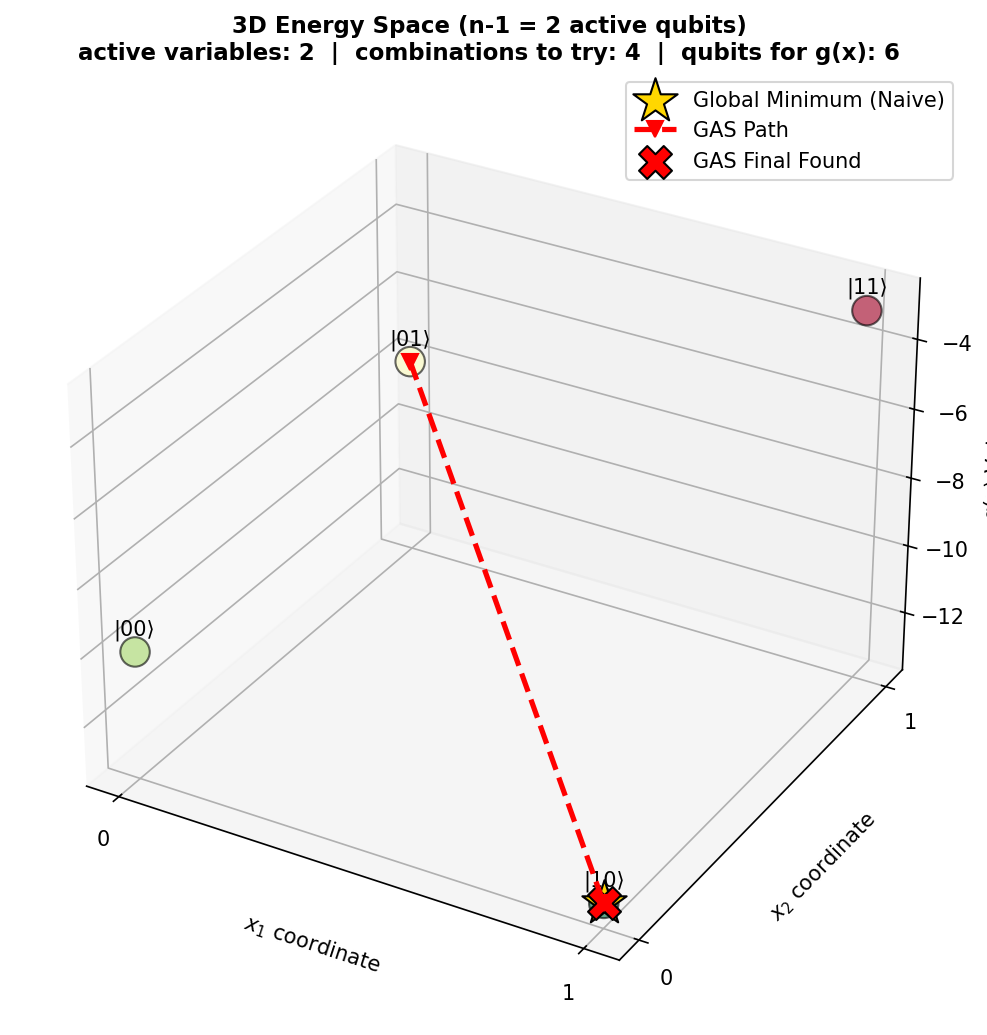
\includegraphics[width=0.35\textwidth]{Code/plots/quadratic_landscape/quadratic_landscape_n3_seed42.png}
  \caption{Cas $n=3$, seed=42 : espace 3D, 4 combinaisons. GAS trouve le minimum global
           en 1 saut depuis le point de départ $|01\rangle$.}
  \label{fig:gas_n3}
\end{figure}

\begin{figure}[H]
  \centering
  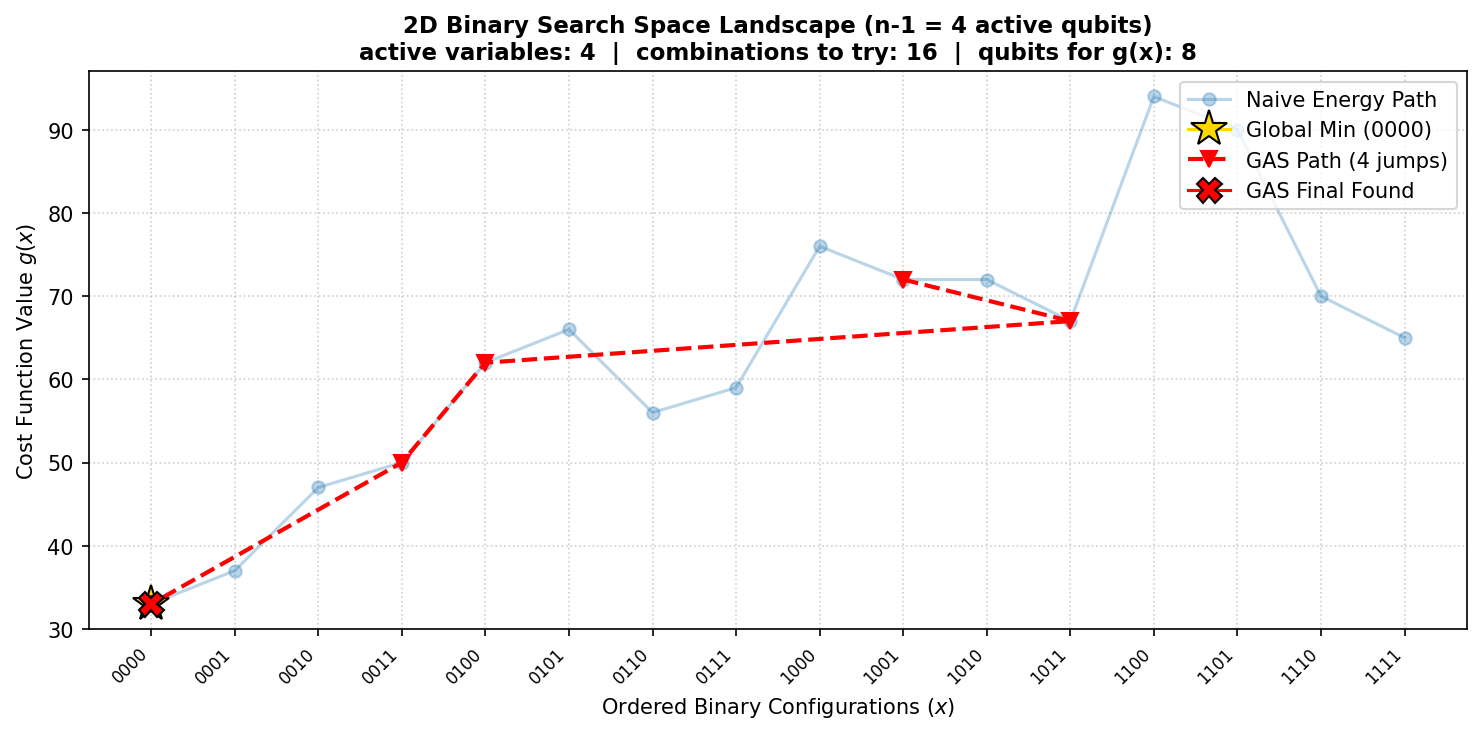
\includegraphics[width=0.65\textwidth]{Code/plots/quadratic_landscape/quadratic_landscape_n5_seed7.png}
  \caption{Cas $n=5$, seed=7 : espace 2D, 16 combinaisons. GAS effectue 3 sauts
           successifs et converge vers le minimum global $|0000\rangle$ ($g=33$).}
  \label{fig:gas_n5}
\end{figure}

\subsubsection{Non-convergence stochastique — cas seed=88}

\begin{figure}[H]
  \centering
  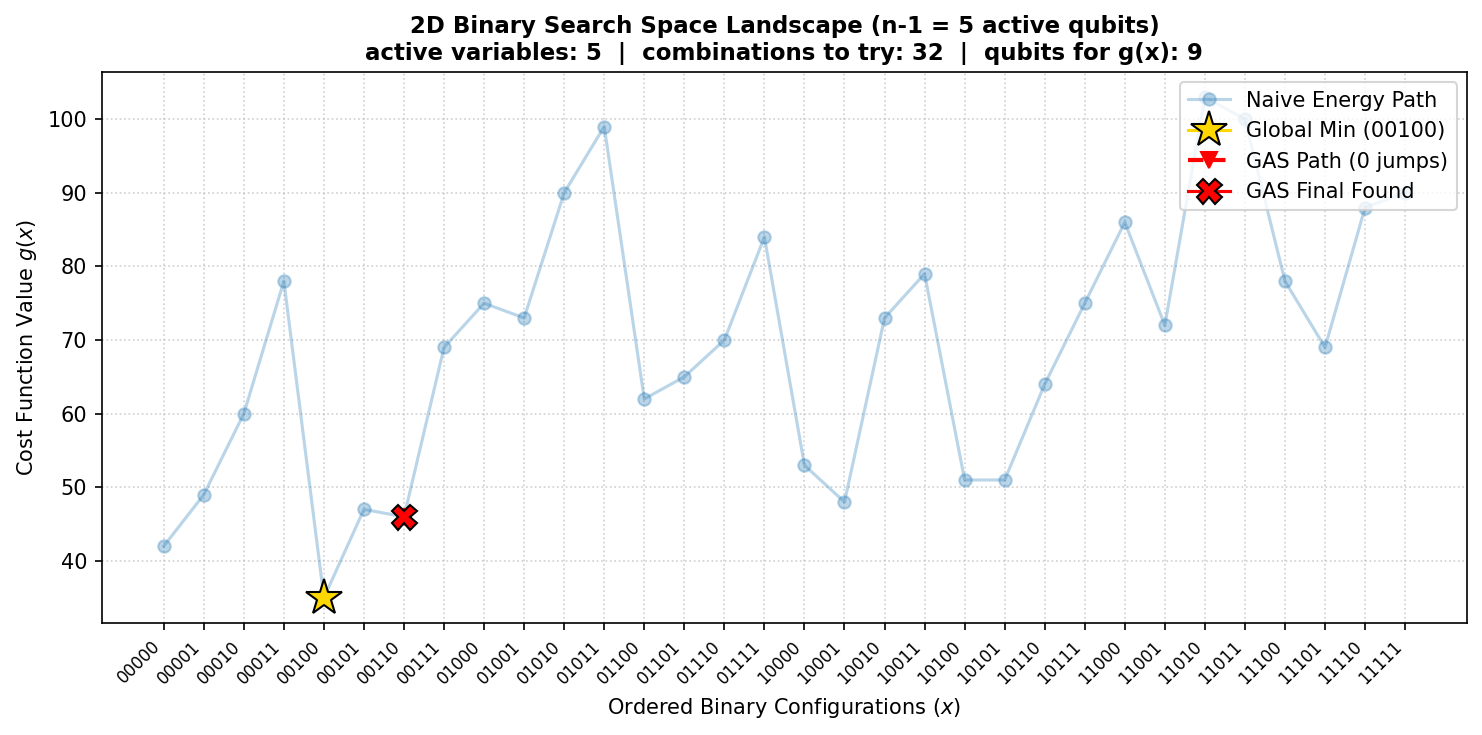
\includegraphics[width=0.65\textwidth]{Code/plots/quadratic_landscape/quadratic_landscape_n6_seed88.png}
  \caption{Cas $n=6$, seed=88 : espace de 32 combinaisons. GAS n'effectue aucun saut
           et s'arrête avec $g(y)=46$, loin du minimum global $g=35$ ($|00100\rangle$).}
  \label{fig:gas_n6}
\end{figure}

Le cas seed=88 (figure~\ref{fig:gas_n6}) illustre un phénomène inhérent à l'algorithme :
la \textbf{non-convergence stochastique}. L'algorithme tourne en boucle ($m$ monte de
$1.0$ à $\sqrt{32} \approx 5.66$ par paliers de $\times 1.2$, soit $\sim$10 tours) sans
jamais mesurer un $x$ tel que $g(x) < g(y_0) = 46$.

Ce n'est pas un bug : avec $t \approx 4$ solutions sur $N=32$ (~12\,\% de l'espace), la
probabilité d'échec à chaque tour est $\geq 3/4$, et la probabilité de tout rater sur
$k$ tours consécutifs est $(3/4)^k$. Pour $k=10$ tours, cela donne $(3/4)^{10} \approx
5.6\,\%$ — un événement rare mais possible. C'est précisément ce que garantit le
théorème BBHT : la convergence est assurée en espérance, non presque sûrement.

La solution préconisée par Dürr et Høyer est de relancer l'algorithme avec un nouveau
$y_0$ aléatoire dès que $m$ atteint $\sqrt{N}$ : chaque redémarrage est indépendant et
la probabilité de rater \emph{tous} les redémarrages décroît exponentiellement.


\newpage

%--------------------------------------------------
\appendix
\section{Calcul de la somme $\displaystyle\sum_{j=0}^{m-1}\cos((4j+2)\theta)$}
\label{ann:bbht}
%--------------------------------------------------

On souhaite calculer $S = \displaystyle\sum_{j=0}^{m-1}\cos\!\bigl((4j+2)\theta\bigr)$.

\medskip\noindent\textbf{Passage aux exponentielles complexes.}
En utilisant $\cos(\varphi) = \mathrm{Re}(e^{i\varphi})$, on écrit :
\[
S = \mathrm{Re}\!\left(\sum_{j=0}^{m-1} e^{i(4j+2)\theta}\right)
  = \mathrm{Re}\!\left(e^{2i\theta}\sum_{j=0}^{m-1} e^{4ij\theta}\right)
\]

\medskip\noindent\textbf{Somme géométrique.}
La somme intérieure est une suite géométrique de raison $r = e^{4i\theta}$ et de premier terme $1$ :
\[
\sum_{j=0}^{m-1} e^{4ij\theta}
= \frac{1 - e^{4im\theta}}{1 - e^{4i\theta}}
\]
On factorise numérateur et dénominateur par leurs demi-angles :
\[
= \frac{e^{2im\theta}\bigl(e^{-2im\theta} - e^{2im\theta}\bigr)}{e^{2i\theta}\bigl(e^{-2i\theta} - e^{2i\theta}\bigr)}
= \frac{e^{2im\theta}\cdot(-2i\sin(2m\theta))}{e^{2i\theta}\cdot(-2i\sin(2\theta))}
= \frac{e^{2im\theta}\sin(2m\theta)}{e^{2i\theta}\sin(2\theta)}
\]

\medskip\noindent\textbf{Calcul de la partie réelle.}
En réinjectant dans $S$ :
\[
S = \mathrm{Re}\!\left(e^{2i\theta}\cdot\frac{e^{2im\theta}\sin(2m\theta)}{e^{2i\theta}\sin(2\theta)}\right)
  = \mathrm{Re}\!\left(\frac{e^{2im\theta}\sin(2m\theta)}{\sin(2\theta)}\right)
  = \frac{\sin(2m\theta)\cos(2m\theta)}{\sin(2\theta)}
\]
En appliquant l'identité de l'angle double $\sin(2m\theta)\cos(2m\theta) = \dfrac{\sin(4m\theta)}{2}$, on obtient :
\[
\boxed{S = \sum_{j=0}^{m-1}\cos\!\bigl((4j+2)\theta\bigr) = \frac{\sin(4m\theta)}{2\sin(2\theta)}}
\]

%--------------------------------------------------
\section{Nombre espéré d'itérations au stade $s$}
\label{ann:esperance}
%--------------------------------------------------

Au stade $s$ de l'algorithme ERS, le paramètre vaut $m = \lambda^{s-1}$. L'indice $j$ est tiré
uniformément dans $\{0,1,\ldots,\lceil m \rceil - 1\}$, qui contient $\lceil m \rceil$ valeurs. Par la formule de Gauss ($\sum_{k=0}^{n-1} k = n(n-1)/2$), le nombre espéré d'itérations de Grover est :
\[
\mathbb{E}[j]
= \frac{0 + 1 + \cdots + (\lceil m \rceil - 1)}{\lceil m \rceil}
= \frac{\lceil m \rceil\,(\lceil m \rceil - 1)/2}{\lceil m \rceil}
= \frac{\lceil m \rceil - 1}{2}.
\]
Or $\lceil m \rceil - 1 < m$ dans tous les cas (strictement, que $m$ soit entier ou non), donc :
\[
\mathbb{E}[j] = \frac{\lceil m \rceil - 1}{2} < \frac{m}{2} = \frac{\lambda^{s-1}}{2}.
\]

\end{document}
